\documentclass[12pt]{article}
\usepackage[utf8]{inputenc}
\usepackage[T1]{fontenc}
\usepackage[brazilian]{babel}
\usepackage{graphicx}
\usepackage{geometry}
\usepackage{setspace}
\usepackage{tikz}
\usetikzlibrary{positioning, arrows.meta}

\geometry{a4paper, margin=2.5cm}
\onehalfspacing

\begin{document}

\begin{titlepage}
\begin{center}
\vspace*{1cm}
{\Large \textbf{UNIVERSIDADE DE SÃO PAULO}}\\[0.5cm]
{\Large \textbf{INSTITUTO DE CIÊNCIAS MATEMÁTICAS E DE COMPUTAÇÃO}}\\[0.5cm]
{\large DEPARTAMENTO DE CIÊNCIAS DE COMPUTAÇÃO}\\[4cm]

{\Large \textbf{Projeto de Pesquisa de Iniciação Científica - Sem Bolsa}}\\[0.5cm]
\rule{\linewidth}{0.5pt}\\[0.5cm]
{\LARGE \textbf{GCN Web Tool}}\\[0.5cm]
\rule{\linewidth}{0.5pt}\\[1.5cm]

\begin{tabular}{ll}
\textit{Candidato:} & \textit{Orientador:} \\[1cm]
\rule{6cm}{0.5pt} & \rule{6cm}{0.5pt} \\
Ian Bezerra & Lucas Pascotti Valem \\
\end{tabular}
\end{center}
\end{titlepage}

\section*{Resumo}

O estudo de 



% Sumário (Table of Contents)
\tableofcontents
\newpage

% Add your report content here
\section{Introdução}
Este relatório apresenta o desenvolvimento da ferramenta web GCN (Graph Convolutional Network).

\section{Trabalhos Relacionados}
% Add your methodology section

\section{Objetivos}
\subsection{Objetivo Geral}

\subsection{Objetivos Específicos}

\section{Plano de Trabalho e cronograma}
\subsection{Pipeline do Projeto}

A Figura \ref{fig:pipeline} ilustra o pipeline completo do projeto, que consiste nas seguintes etapas:
\begin{figure}[h]
    \centering
    \begin{tikzpicture}[node distance=2cm, auto, thick]
        % Nodes
        \node[draw, rectangle, minimum width=3cm, minimum height=1cm] (alexnet) {CNN};
        \node[draw, rectangle, minimum width=3cm, minimum height=2.5cm, right=of alexnet] (embeddings) {};
        \node[draw, rectangle, minimum width=4cm, minimum height=2.5cm, right=of embeddings] (distance) {};
        
        \node[draw, rectangle, minimum width=3cm, minimum height=2cm, below=of embeddings] (rankings) {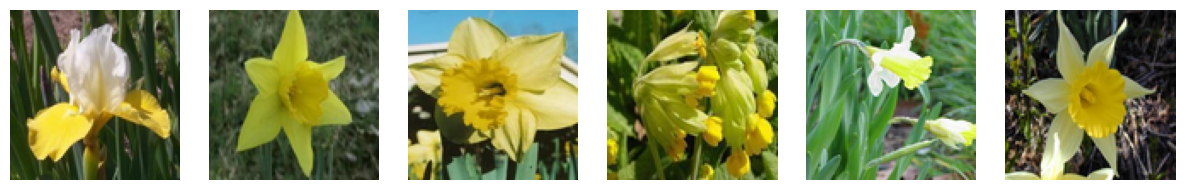
\includegraphics[width=2.8cm]{rankings.png}};
        \node[draw, rectangle, minimum width=3cm, minimum height=1cm, right=of rankings] (graph) {Grafo};
        
        % Arrows
        \draw[->] (alexnet) -- (embeddings);
        \draw[->] (embeddings) -- (distance);
        \draw[->] (distance) -- (rankings);
        \draw[->] (rankings) -- (graph);
        
        % Embeddings visualization with vectors in the top part of the embeddings box
        \begin{scope}[shift={(embeddings.north)}, yshift=-1.2cm, scale=0.4]
            % Coordinate system
            \draw[->] (-1.5,0) -- (1.5,0) node[right] {$x$};
            \draw[->] (0,-1.5) -- (0,1.5) node[above] {$y$};
            
            % Vectors
            \draw[->, thick, blue] (0,0) -- (0.8,1.2) node[right] {$v_1$};
            \draw[->, thick, red] (0,0) -- (-0.7,0.9) node[left] {$v_2$};
            \draw[->, thick, green] (0,0) -- (1.1,0.3) node[right] {$v_3$};
            \draw[->, thick, orange] (0,0) -- (-0.5,-0.8) node[left] {$v_4$};
        \end{scope}
        
        % Distance matrix visualization
        \begin{scope}[shift={(distance.north)},xshift=-0.5cm, yshift=-1.9cm, scale=0.35]
            % Matrix
            \draw (0,0) grid (4,4);
            
            % Values in the matrix (darker colors for smaller distances)
            \fill[fill=white!80!black] (0,0) rectangle (1,1);
            \fill[fill=white!30!black] (0,1) rectangle (1,2);
            \fill[fill=white!10!black] (0,2) rectangle (1,3);
            \fill[fill=white!100!black] (0,3) rectangle (1,4);
            
            \fill[fill=white!20!black] (1,0) rectangle (2,1);
            \fill[fill=white!80!black] (1,1) rectangle (2,2);
            \fill[fill=white!100!black] (1,2) rectangle (2,3);
            \fill[fill=white!40!black] (1,3) rectangle (2,4);
            
            \fill[fill=white!5!black] (2,0) rectangle (3,1);
            \fill[fill=white!100!black] (2,1) rectangle (3,2);
            \fill[fill=white!80!black] (2,2) rectangle (3,3);
            \fill[fill=white!15!black] (2,3) rectangle (3,4);
            
            \fill[fill=white!100!black] (3,0) rectangle (4,1);
            \fill[fill=white!25!black] (3,1) rectangle (4,2);
            \fill[fill=white!35!black] (3,2) rectangle (4,3);
            \fill[fill=white!80!black] (3,3) rectangle (4,4);
            % Draw grid lines again to make them visible
            \draw (0,0) grid (4,4);
            
            % Labels
            \node at (-0.5, 0.5) {$v_4$};
            \node at (-0.5, 1.5) {$v_3$};
            \node at (-0.5, 2.5) {$v_2$};
            \node at (-0.5, 3.5) {$v_1$};
            
            \node at (0.5, 4.5) {$v_1$};
            \node at (1.5, 4.5) {$v_2$};
            \node at (2.5, 4.5) {$v_3$};
            \node at (3.5, 4.5) {$v_4$};
        \end{scope}
        
        % Text at the bottom of the embeddings box
        \node at (embeddings.south) [yshift=0.4cm] {Embeddings};
        
        % Text at the bottom of the distance matrix box
        \node at (distance.south) [yshift=0.4cm] {Matriz de Distância};
        
        % Text at the bottom of the rankings box
        \node at (rankings.south) [yshift=0.4cm] {Rankings};
    \end{tikzpicture}
    \caption{Pipeline do projeto: da extração de características com CNN até construção do grafo}
    \label{fig:pipeline}
\end{figure}

O pipeline começa com a extração de características das imagens utilizando a rede neural convolucional AlexNet, gerando embeddings (representações vetoriais) para cada imagem. Em seguida, calculamos a matriz de distância entre esses embeddings, que é usada para gerar rankings de similaridade. Por fim, esses rankings são utilizados para construir o grafo que representa as relações entre as imagens.


% Add your methodology section

\section{Materiais e métodos}
% Add your results section

\section{Referências}
% Add your conclusion

\end{document}
